\newpage
\chapter{An implementation of DRMM}

The implementation and evaluation of this Neural IR system were divided in five macro tasks:

\begin{itemize}
\item preprocessing and analysis of dataset (Robust04 \cite{rob04});
\item implementation of the model;
\item replication;
\item evaluation of results;
\item discussion.
\end{itemize}

The rest of this chapter describes and analyzes each task in detail.

\section{Preliminar Analysis}

Before (and while) implementing DRMM I considered different options available regarding all the four previous steps.\\

\textbf{Collection preprocessing}:

\begin{itemize}
 \item the corpus and queries can be stemmed/not stemmed, processed with
stopwords/without stopwords, and different fields (or combination of them) from topics can be considered (i.e. title and description);
 \item the preranked results can be obtained with a wide range of retrieval models. For instance, the authors of the original paper use Bm25 and QL models as first-stage rankers.
\end{itemize}

\textbf{DRMM system}:

\begin{itemize}
 \item the size of the word embeddings may vary;
 \item the query term gating can take as input the query embeddings or the query terms IDF;
 \item the hyperparameters of the model need to be tuned (i.e. number of epochs, learning rate, early stopping, batch size).
\end{itemize}

After considering the above options, I chose the following configuration for my tests:
both corpus text / query titles stemmed and without stopwords; the top 2000 preranked results with both QL and Bm25 retrieval algorithms, 300 embeddings size, and training/testing on all histograms mode/term gating network.

Despite a few hyperparameters of the model were given in \cite{drmm}, I had to (empirically) try all the others (e.g. number of epochs, number of documents to sample from the training set, initial learning rate and early stopping values).

The workflow that I followed for my implementation is reported in the following picture:

\begin{adjustbox}{width=6.5in,totalheight=5in, center}
\begin{tikzpicture}[node distance = 3.7cm, auto]
    % Place nodes
    \node [block] (pre) {Tokenization};
    \node [block, right of=pre] (swr) {Stopwords removal};
    \node [block, right of=swr] (st) {Stemming};
    \node [block, right of=st] (emb) {Word embeddings generation};
    \node [cloud, above of=swr] (inquery) {INQUERY \\ stoplist};
    \node [cloud, above of=st] (krovetz) {Krovetz stemmer};
    \node [cloud, above of=emb] (w2v) {Word2Vec};
    \node [decision, below of=swr, node distance = 5cm] (decide) {Term gating function};
    \node [block, below of=decide, node distance = 4cm] (idf) {Idf computation};
    \node [block, right of=decide, node distance = 7cm] (hist) {Histograms CH generation};
    \node [block, right of=hist] (ids) {Generate positive/negative samples for training};
    \node [decision, below of=ids, node distance = 4.5cm] (decidehist) {Histograms modalities};
    \node [block, right of=decidehist, node distance = 4cm] (nh) {Normalize histograms by sum};
    \node [block, left of=decidehist, node distance = 4cm] (lch) {Normalize histograms by logarithm};
    \node [block, below of=decidehist] (drmm) {Run DRMM};
    % Draw edges
    \draw [cm dotted,line width=.2mm,step=.5] (swr) -- (inquery);
    \draw [cm dotted,line width=.2mm,step=.5] (st) -- (krovetz);
    \draw [cm dotted,line width=.2mm,step=.5] (emb) -- (w2v);
    \path [line] (pre) -- (swr);
    \path [line] (swr) -- (st);
    \path [line] (st) -- (emb);
    \path [line] (emb.south) -- ++(0,-2) -| (decide.north);
    \path [line] (emb.south) -- ++(0,-2) -| (decide.north);
    \path [line] (decide) -- node {idf} (idf);
    \path [line] (idf) -- (hist);
    \path [line] (decide) -- node {query terms}(hist);
    \path [line] (ids.south) |- (decidehist.north);
    \path [line] (decidehist) -- node {NH}(nh);
    \path [line] (decidehist) -- node {LCH}(lch);
    \path [line] (hist) -- (ids);
    \path [line] (nh.south) |- (drmm.east);
    \path [line] (lch.south) |- (drmm.west);
\end{tikzpicture}
\end{adjustbox}

The time required for each of the previous steps is reported in the following table:

\begin{table}[h!]
\centering
 \begin{tabular}{cc} 
 \hline
 Process & Time (mm:ss) \\
 \hline
 Tokenization/data cleaning & 35:13 \\
 Stopwords removal & 01:31 \\
 Stemming & 01:05 \\
 Word embeddings generation & 11:25 \\
 Idf computation & 00:50 \\
 Histograms computation and saving & 03:07 \\
 Running 5-fold cross validation & $\sim$ 44:00 (w/o considering early stopping) \\
 \hline
 \end{tabular}
 \caption{Computing time required on a pc with the following specifications: 31GiB of system memory, processor: Intel(R) Core(TM) i7-8700 CPU @ 3.20GHz, graphic card: NVIDIA Quadro M4000}
 \label{table:timeit}
\end{table}

\subsection{Experimental collection}

The goal of the TREC Robust track (\cite{rob04}) is to improve the consistency of retrieval
technology by focusing on the most difficult topics.

The document collection for the Robust track is the set of documents from both TREC Disks 4 and 5 minus the the Congressional Record on disk 4.\\

\textbf{Trec format}\\

There are 2 formats, depending on the type of document (pure text or HTML).\\

\begin{lstlisting}
<DOC>
	<DOCNO> document_number </DOCNO>
	Here there could be tags like Title, Author, Profile, Headline, Date, Page...
	<TEXT> (plain text or HTML format)
		Document text
	</TEXT>
</DOC>
\end{lstlisting}

\textbf{Topics}\\

TREC calls a natural language statement representing an information need a ``topic'' to distinguish it from a ``query'', which is the portion of text actually presented to the retrieval system.

The topics are formatted using a very simple SGML (Standard Generalized Markup Language) style tagging (different than XML format).\\

An example taken from Robust04:\\

\lstset{language=XML,basicstyle=\ttfamily,breaklines=true}

\begin{lstlisting}
<top>
	<num> Number: 301
	<title> International Organized Crime
	<desc> Description: Identify organizations that participate in international criminal activity, the activity, and, if possible, collaborating organizations and the countries involved.
	<narr> Narrative: A relevant document must as a minimum identify the organization and the type of illegal activity (e.g., Columbian cartel exporting cocaine). Vague references to international drug trade without identification of the organization(s) involved would not be relevant.
</top>
\end{lstlisting}

\textbf{Relevance Judgements}\\

The format of a relevance judgment (qrels) file is the following:

\begin{itemize}
\item TOPIC: topic number;
\item ITERATION: feedback iteration (almost always zero and not used);
\item DOCUMENT\#: official document number that corresponds to the docno field in the documents;
\item RELEVANCY: binary code of 0 for not relevant docs and 1 for relevant docs.
\end{itemize}

\textbf{Qrel row example}: ``301 0 FBIS3-10082 1''

Documents not occurring in the relevance judgements file were not judged by the human assessor and are \textbf{assumed to be non relevant} in the evaluations used in TREC.

In a qrels file the human assessors are told to judge a document relevant if any
piece of the document is relevant (regardless of how small the piece is in
relation to the rest of the document). Thus, judgements have been given under the \textbf{scope hypothesis}.

\section{Ad-Hoc Information Retrieval on TREC Robust04}
\label{sec:leaderboadrobust04}

DRMM is not the first (Neural) IR model to evaluate its performance on TREC Robust 2004 track (\cite{rob04}). In fact, during past years, others retrieval models have been tested against this collection.

\begin{figure}[H]
  \centering
  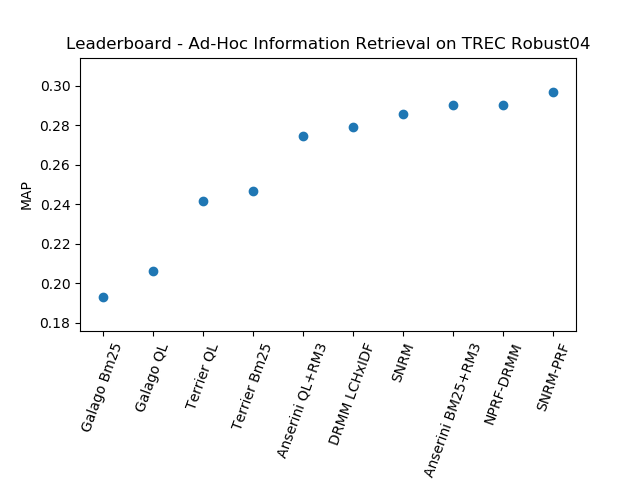
\includegraphics[width=0.8\textwidth]{res/img/EvalRobust04.png}
  \caption{Ad-Hoc Information Retrieval on TREC Robust04}
  \label{fig:evalRob04}
\end{figure}

The above picture reports the state-of-the-art leaderboard of ad-hoc retrieval on the TREC Robust04 collection \footnote{\url{https://paperswithcode.com/sota/ad-hoc-information-retrieval-on-trec-robust04}}.
QL and Bm25 are two traditional IR models and RM3 is a relevance-based model, that provide a solid baseline while all the others are recent Neural IR models (described in \ref{ssec:historyNeuIR}).

\begin{table}[H]
\centering
\begin{tabular}{ccccc}
\textbf{Method} & \textbf{MAP} & \textbf{P@20} & \textbf{nDCG@20} & \textbf{Year} \\ \hline
Anserini BM25+RM3 & 0.290 & \textit{Not available} & \textit{Not available} & 2018 \\ \hline
Anserini QL+RM3 & 0.274 & \textit{Not available} & \textit{Not available} & 2018 \\ \hline
SNRM & 0.285 & 0.376 & 0.431 & 2018 \\ \hline
SNRM-PRF & 0.297 & 0.394 & 0.439 & 2018 \\ \hline
NPRF-DRMM & 0.290 & 0.406 & 0.45 & 2018 \\ \hline
DRMM & 0.279 & 0.382 & 0.431 & 2017 \\ \hline
\end{tabular}
\caption{State of the art of ad-hoc retrieval on TREC Robust04}
\label{table:leaderboardRob04}
\end{table}


\section{Dataset analysis}

Preprocessing steps:

\begin{itemize}
\item Parsing of collection and topics;
\item Indexing of parsed collection and queries with Terrier Dirichlet QL and Bm25 algorithms (to obtain preranked data);
\item Stemming and stopwords removal;
\item Word-embeddings preparation both for collection and queries with Word2Vec (although queries-based embeddings were ignored) - this is where originates the out-of-vocabulary problem;
\item Pre-computed IDF values for each query term (input to query term gating);
\item Subdivision of ground truth labels (based on topics) for k-fold cross validation.
\end{itemize}

\subsection{Parsing of documents and topics}

For documents, the following attributes were considered: docno, headline and text, whereas for topics only the title attribute was considered.

Both documents and queries were lower-cased, punctuation and any non-alphabetic characters (including numbers and words that contain numbers) were removed along with every tag and HTML entities such as \&lg, \&gt etc.

Example of sentence cleaning:

``BOOK REVIEW; A SURVIVOR'S ACCOUNT OF BRAIN SURGERY A Bomb in the Brain: A Heroic Tale of Science, Surgery and Survival'' becomes ``book review a survivors account of brain surgery a bomb in the brain a heroic tale of science surgery and survival''.

\subsection{Indexing of parsed collection and queries}

Indexing was performed both with Galago and Terrier search engines using the krovetz stemmer and the INQUERY stoplist. The original paper performed stopwords removal only on queries, but I performed it also on the entire text collection, in order to remove noisy words.

\subsection{Data preliminar analysis}

The following tables and plots report statistics on unique (vocabulary) words per documents and per queries.

\begin{table}[H]
\centering
\begin{tabular}{p{2cm}p{1.5cm}p{2cm}ccccccc}
 & Stemmed & Stopwords removal & Min & Max & Mean & Median & Mode & Std \\ \hline
Doc. vocabulary length & & & 1 & 13779 & 211.05 & 170 & 89 & 168.81 \\ \hline
Queries vocabulary length & & & 1 & 5 & 2.7 & 3 & 3 & 0.704 \\ \hline
Doc. vocabulary length & & x & 1 & 13725 & 158.44 & 122 & 56 & 141.19 \\ \hline
Queries vocabulary length & x & x & 1 & 4 & 2.62 & 3 & 3 & 0.65 \\ \hline
Doc. vocabulary length & x & x & 1 & 13409 & 148.42 & 116 & 54 & 127.23 \\ \hline
Queries vocabulary length & x & x & 1 & 4 & 2.62 & 3 & 3 & 0.65 \\ \hline
\end{tabular}
\caption{Data statistics}
\label{table:DataMeasures}
\end{table}

As it can be understand from the statistics, the length of documents vocabulary is not uniform throughout the corpus. Most of them are, in fact, far from the average-length. Queries, instead, have a vocabulary length between one and four words. 

\begin{figure}[!tbp]
  \centering
  \subfloat[Length of vocabularies per document (corpus without stopwords and stemmed)]{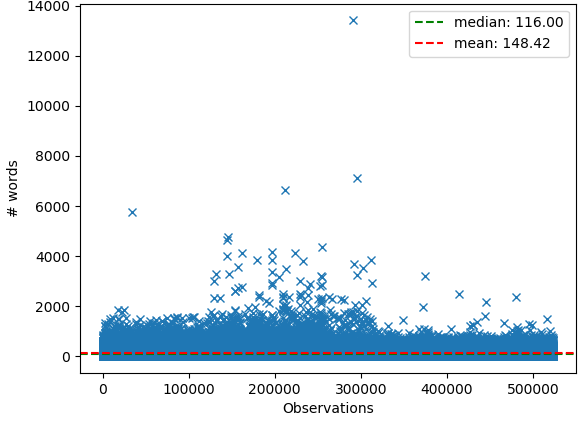
\includegraphics[width=0.5\textwidth]{corpus_docs_words_ssr.png}\label{fig:f1}}
  \hfill
  \subfloat[Length of vocabularies per queries (without stopwords and stemmed]{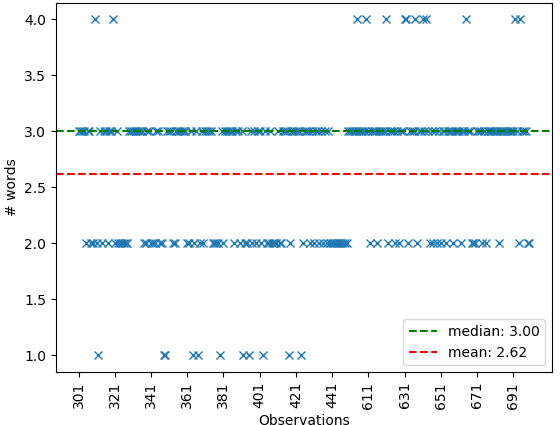
\includegraphics[width=0.5\textwidth]{queries_words_ssr.png}\label{fig:f2}}
  \caption{Histograms count-based}
  \label{fig:vocab_documents}
\end{figure}

These statistics shows that the stopwords and the stemming components are reducing the length of both documents and queries vocabularies.

\begin{table}[H]
\centering
\begin{tabular}{p{2cm}p{2cm}p{2cm}c}
 & Stemmed & Stopwords removal & Count \\ \hline
Docs words & & & 110563253 \\ \hline
Queries words & & & 3624 \\ \hline
Docs words & & x & 83003929 \\ \hline
Queries words & & x & 2131 \\ \hline
Docs words & x & x & 77750991 \\ \hline
Queries words & x & x & 2063 \\ \hline
\end{tabular}
\caption{Data words count}
\end{table}

Guo et al. reported their statistics on the original paper for the test collection, after preprocessing:

\begin{table}[H]
\centering
\begin{tabular}{ccc}
 & Theirs & Mine \\ \hline
Vocabulary & 0.6M & 509731 \\
Document Count & 0.5M & 523857 \\
Query Count words & 250 & 250 \\ \hline
\end{tabular}
\caption{Data words count}
\end{table}

My vocabulary has less words than theirs because I performed stopwords removal on the full corpus of documents, not just on queries.

\subsection{Word-embeddings training with Word2Vec}
\label{ssec:wemb}

I used the Gensim implementation of Word2Vec \footnote{\url{https://radimrehurek.com/gensim/models/word2vec.html}} with the following parameters:

\begin{table}[H]
\centering
\begin{tabular}{p{8cm}|c}
\multicolumn{2}{c}{\textbf{Word2Vec}} \\
Parameters & Value \\ \hline
Algorithm & CBOW \\
Dimension of term embeddings & 300 \\
Context window size & 10 \\
Negative samples per word & 10 \\
Sampling threshold (subsampling of frequent words) & $10^{-4}$ \\
Minimum word count (words with frequency < 10 are not considered) & 10 \\ \hline
\end{tabular}
\caption{Parameters configuration for Word2Vec}
\label{table:w2v_config}
\end{table}

Each document in the corpus was given in input to Word2Vec as a string. Alternatively, a document could have been given in input as a list of sentences. Later, I will show results for both choices.

If a word is present only in a query and not in the corpus, that word is considered out-of-vocabulary.

\subsection{A quick inspection of word embeddings}

The vocabulary of Word2Vec model contains less words than the vocabulary of the collection, because all words that occurs less than 10 times are removed.

At this point, in the pipeline that builds the input to DRMM, the ``words out-of-vocabulary'' problem originates. That is, some words present in the collection have not a corresponding embedding. DRMM alleviate this problem by allowing exact matching between these words left out.

\begin{table}[H]
\centering
\begin{tabular}{p{2cm}p{2cm}p{4cm}p{4cm}}
\textbf{stemming} & \textbf{stopwords removal} & \textbf{Original corpus vocabulary size} & \textbf{Word2Vec model vocabulary size} \\ \hline
& & 629164 & 145226 \\
& x & 628751 & 144834 \\
x & x & 509731 & 110158 \\
\end{tabular}
\caption{Word counts}
\end{table}

In the following, I report a simple look up of the top 6 most similar words for ``night'', with the respective cosine similarity, for all cases (unstemmed + no stopwords removal; unstemmed + stopwords removal; stemmed + stopwords removal).

Cosine similarity function (equation \ref{eq:cosine}) measures the cosine of the angle between two vectors and returns value in the interval $[-1, 1]$. If two vectors are parallel/orthogonal, their cosine similarity is +1/0. When they are opposite, their cosine similarity is -1.

\begin{table}[H]
\centering
\begin{tabular}{ll}
\textbf{Similar words} & \textbf{Cosine similarity} \\ \hline  
nights & 0.745 \\
evening & 0.736\\
morning & 0.657 \\
afternoon & 0.619 \\
afternoons & 0.584 \\
weekend & 0.574 \\
\end{tabular}
\caption{Lookup word: ``night''; unstemmed corpus without stopwords removal}
\end{table}

\begin{table}[H]
\centering
\begin{tabular}{ll}
\textbf{Similar words} & \textbf{Cosine similarity} \\ \hline  
evening & 0.777 \\
nights & 0.770 \\
morning & 0.699 \\
afternoon & 0.642 \\
midnight & 0.620 \\
sunday & 0.597 \\
\end{tabular}
\caption{Lookup word: ``night''; unstemmed corpus with stopwords removal}
\end{table}

\begin{table}[H]
\centering
\begin{tabular}{ll}
\textbf{Similar words} & \textbf{Cosine similarity} \\ \hline  
evening & 0.779 \\
nights & 0.755 \\
morning & 0.719 \\
afternoon & 0.651 \\
midnight & 0.631 \\
sunday & 0.607 \\
\end{tabular}
\caption{Lookup word: ``night''; stemmed corpus with stopwords removal}
\end{table}

It can be noticed that, when stopwords removal and stemming are applied, the order of the results changes. Moreover, words as ``evening'', ``morning'', ``midnight'' and ``sunday'' get a closer (textual) position to the word ``night'' and their cosine similarity increases.

I also inspect the in-out embeddings (cited in \cite{Mitra2016ADE}) of the trained Word2Vec model.

As previously mentioned, Word2Vec model contains two separate embedding spaces (in and out) whose interactions capture additional distributional semantics of words that are not observable by considering them separately.

The results were as follows:

\begin{table}[H]
\centering
\begin{tabular}{cc}
\hline
\textbf{night} & \textbf{Cosine similarity} \\ \hline
sleepless & 0.102 \\
saturday & 0.096 \\
sunday & 0.089 \\
night & 0.085 \\
monday & 0.082\\
\hline
\end{tabular}
\caption{Lookup word: ``night'' (in embedding space for query, out embedding space for corpus); stemmed corpus with stopwords removal}
\label{tab:embsim2}
\end{table}

Words that appear in similar contexts get pushed closer to each other within the in and the out embedding spaces (in-in/out-out) (typical similarity), while in-out (out-in) cosine similarities are higher for words that co-occur often in the training corpus (topically similar). In fact, in table \ref{tab:embsim2} there are some words that do not appear in the previous tables (e.g. ``sleepless'', ``night'', ``monday'').

This is the reason why the results of the table \ref{tab:embsim2} are different from the previous ones.

\subsection{Word embeddings matching signals analysis}

Histograms in DRMM are generated based on the cosine similarity between word embeddings of a query and a document (see section \ref{ssec:mhist}).

Figure \ref{fig:cos_sim_sample} shows the cosine similarity results between the query for ``international organized crime'' and a portion of a document in the collection.

A bin $i$,$j$ in the matrix correspond to the cosine similarity between the embedding vector for the query term $i$ and the document term $j$.

It can be noticed that the query term embedding ``crime'' has an high cosine similarity with terms embeddings of ``evidence'', ``drug'', ``traffick'', ``mafia'' and ``justice''.

This happens because Robust04 \cite{rob04} is a news collection and ``crime'' co-occurs with all of these terms.

\begin{figure}[H]
  \centering
  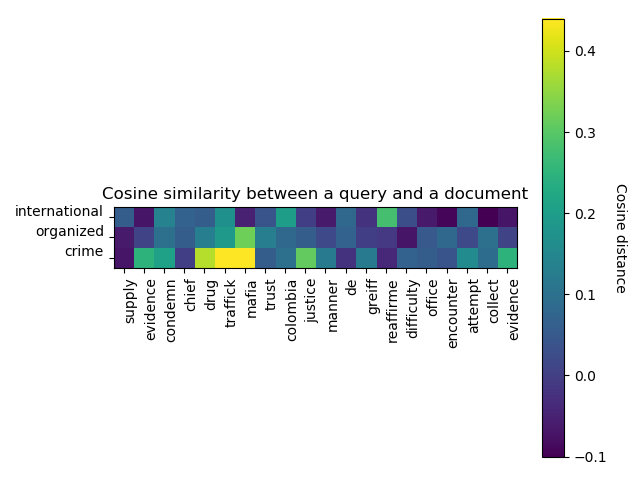
\includegraphics[width=0.9\textwidth]{cos_sim_sample.png}
  \caption{Cosine similarity between query terms and a slice of document}
  \label{fig:cos_sim_sample}
\end{figure}

Next, I give some example of histograms, with respect to the title of topic 301 and two documents, relevant and non relevant. I chose two documents where it can be clearly seen that the matching signals distribution between the relevant and the non relevant is different.

Both document and query were stemmed and without stopwords. For each query term, there is a row of 30 bins (colored different, according to their frequency). Each bin contains a specific similarity range, for
example the ones at the middle (0-($\sim$) 0.067) indicate how many words in the document are orthogonal to the query term; the ones on the right (left) indicate how many words are closer (``opposite'') to the query term.

Note that Word2Vec does not capture antonymy, so opposite vector embeddings are \textbf{not} semantically opposite, which is counter-intuitive.

\begin{figure}[H]
  \centering
  \subfloat[Positive document histograms]{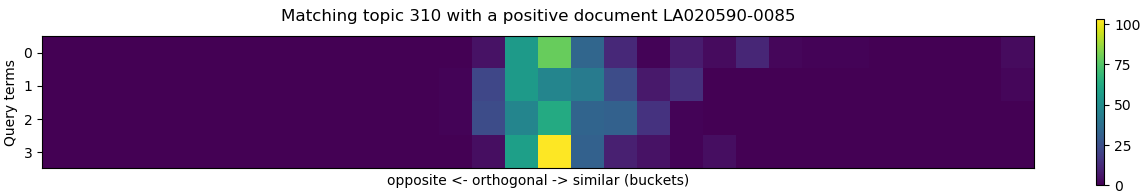
\includegraphics[width=0.8\textwidth]{positive_ch.png}\label{fig:posch}}
  \hfill
  \subfloat[Negative document histograms]{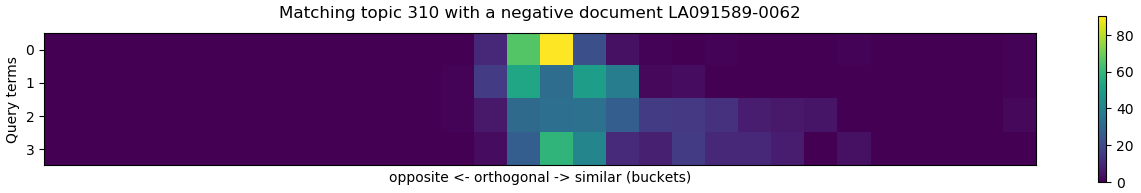
\includegraphics[width=0.8\textwidth]{negative_ch.png}\label{fig:negch}}
  \caption{Count-based istograms}
  \label{fig:hist_ex}
\end{figure}

In the following example, each histogram has been normalized by sum, in fact
the range of values is smaller than the previous example.

\begin{figure}[H]
  \centering
  \subfloat[Positive document histograms]{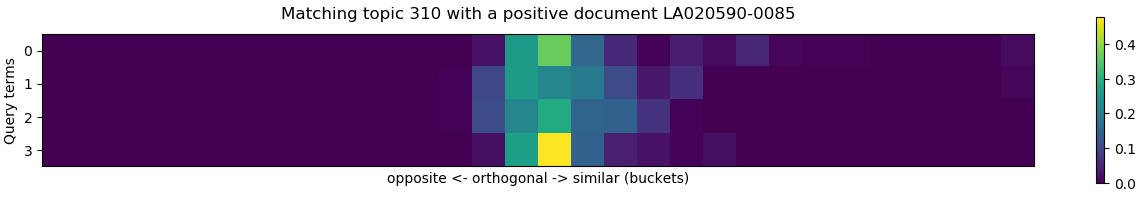
\includegraphics[width=0.8\textwidth]{positive_nh.png}\label{fig:posnh}}
  \hfill
  \subfloat[Negative document histograms]{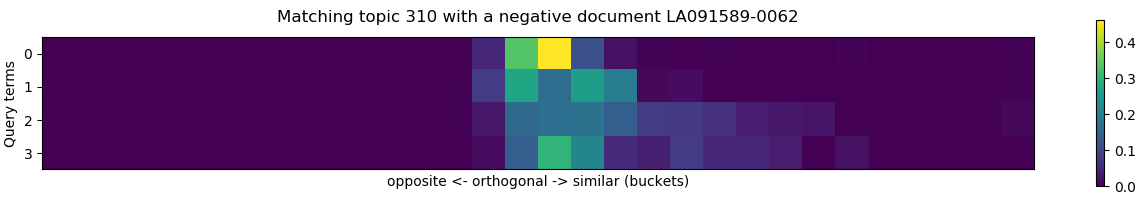
\includegraphics[width=0.8\textwidth]{negative_nh.png}\label{fig:negnh}}
  \caption{Histograms normalized by sum}
  \label{fig:hist_nh_ex}
\end{figure}

The last case is logarithm-based histograms. Matching signals stand out more in this case.

\begin{figure}[H]
  \centering
  \subfloat[Positive document histograms]{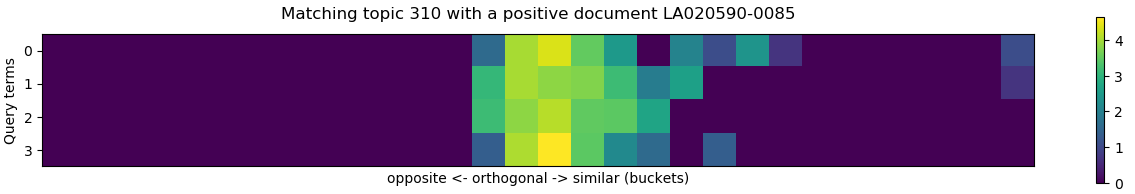
\includegraphics[width=0.8\textwidth]{positive_lch.png}\label{fig:poslch}}
  \hfill
  \subfloat[Negative document histograms]{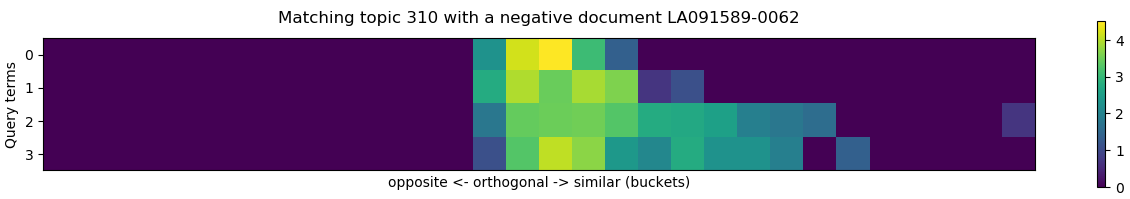
\includegraphics[width=0.8\textwidth]{negative_lch.png}\label{fig:neglch}}
  \caption{Histograms normalized by logarithm}
  \label{fig:hist_lch_sample}
\end{figure}

\subsection{Generation of histograms pair}

All pair query/document from preranked results were considered and their histograms were taken as input to the feed forward neural network.

Histograms generation is a computationally expensive operation, which can be done offline (before training DRMM). Since the moment that this can save a lot of time, I chose to do it in my implementation (although it came with a disk space cost: saving the histograms for the whole corpus (Robust04 \cite{rob04}) required up to 0.5GB).

\section{Evaluation and metrics}
\label{sec:comparison}

For all the deep matching models Guo et al. (\cite{drmm}) adopted a re-ranking strategy for efficient computation.

An initial retrieval was performed using two open-source search engines, Terrier and Galago, to obtain the top 2000 ranked documents (pre-ranked documents) for each topic.

The following table reports the evaluation results for the pre-ranked runs used in \cite{drmm} by Guo et al. and the evaluation results for mine:

\begin{table}[H]
\centering
\begin{tabular}{c|ccc}
Method & MAP & nDCG\@20 & P\@20 \\ \hline
Galago DirichletLM($\mu=1500$) & 0.206 & 0.390 & 0.326 \\
Galago Bm25($k_1 = 1.2, k_3 = 1.0, b=0.75$) & 0.193 & 0.377 & 0.319 \\
Terrier DirichletLM($\mu=2500$) & 0.241 & 0.404 & 0.343 \\
Terrier Bm25($k_1 = 1.2, k_3 = 8d, b = 0.75d$) & 0.247 & 0.417 & 0.359 \\
Original QL(\textit{unknown parameters}) & 0.253 & 0.415 & 0.369 \\
Original Bm25(\textit{unknown parameters}) & 0.255 & 0.418 & 0.370
\end{tabular}
\caption{Evaluation of preranked results}
\end{table}

I chose to use the retrieval results which performance were closer to the original (Terrier runs).

As Guo pointed out in an issue in MatchZoo \footnote{\url{https://github.com/NTMC-Community/MatchZoo/issues/604}}, on Robust04 dataset there is a data imbalance problem, in fact the number of labelled documents for each topic is significantly different from one another.
In this way, the model could be dominated by a specific topic.
Figure \ref{fig:queries_frequencies_bm} shows the (logarithmically scaled) distribution of documents retrieved by Bm25 per topic. It can be noticed that there is also a different distribution of positive and negative examples.
For instance, QL algorithm, on average, retrieves only 3.68\% of positive samples for each topic (with some topics with 0 positive samples - e.g. topic 672) while Bm25 retrieves on average 3.70\% positive samples per topic.
Since the moment that the distributions relative to the runs obtained with these two algorithms are very similar, just the one relative to Bm25 is shown.

\begin{figure}[H]
  \centering
  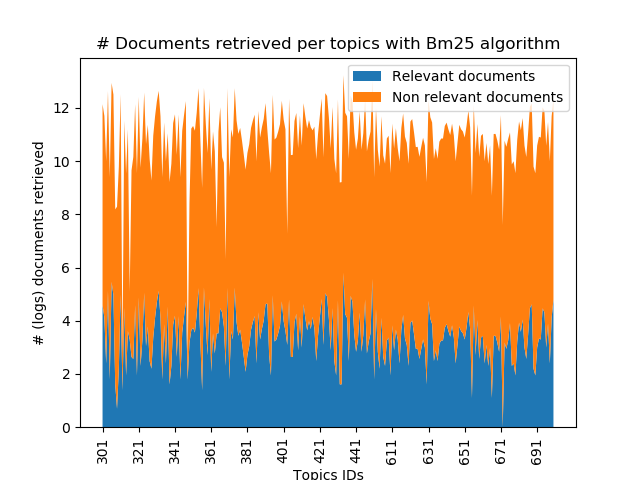
\includegraphics[width=0.7\textwidth]{queries_frequenciesBm25.png}
  \caption{Queries imbalance problem - Bm25 algorithm}
  \label{fig:queries_frequencies_bm}
\end{figure}

\section{5-fold cross validation and parameters tuning}

Guo et al. conducted 5 fold cross validation, to minimize overfitting on topics.

The 250 topics were divided into 5 folds. Each training phase was conducted with documents sampled from 4 folds and the fold left out was used as test set.

Each test fold contains approximately (due to the query imbalance problem, explained in the previous section) $2000 \cdot 50 = 100000$ documents.

At the end of each training phase, the model weights were re-initialized.

\section{DRMM model configuration}

Picture \ref{fig:model_drmm} shows the graph of DRMM. It consists of:

\begin{itemize}
 \item a feed forward ``matching'' neural network for histograms (see equation \ref{eq:lthdenselayer});
 \item a term gating network for each query term (with query term embedding or idf as weight), which use the softmax as ``gating'' function (see equation \ref{eq:aggscore});
 \item the final output, computed as stated in equation ``\ref{eq:drmm_score}'';
 \item the computation of the loss function (see equation \ref{eq:hinge}).
\end{itemize}

\begin{figure}[H]
  \centering
  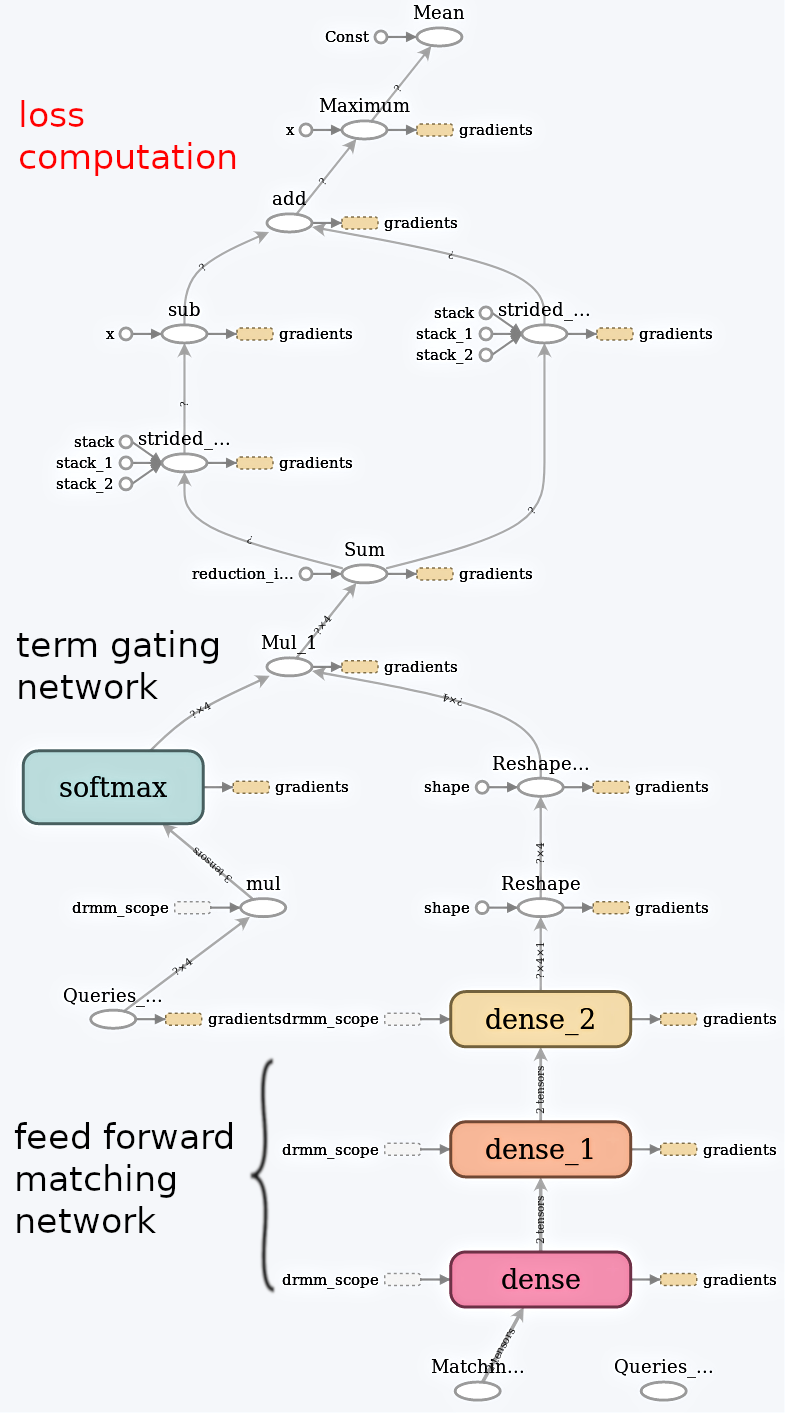
\includegraphics[width=0.8\textwidth]{graphBF2.png}
  \caption{DRMM model (tensorflow graph)}
  \label{fig:model_drmm}
\end{figure}

\subsection{Neural network configuration for experiment}

For each of the experiments, DRMM feed forward neural network used the following parameters (some of them were empirically chosen):

\begin{table}[H]
\centering
\begin{tabular}{p{8cm}|p{5cm}}
\multicolumn{2}{c}{\textbf{DRMM configuration}} \\
Parameters & Value \\ \hline
Number of epochs & 20 \\
Mini batches size & 20 \\
Initial weights & glorot uniform initializer \footnote{draws samples from a uniform distribution within [-limit, limit] where limit is $\sqrt{\frac{6}{fan\_in + fan\_out}}$, fan\_in is the number of input units in the weight tensor and fan\_out is the number of output units in the weight tensor.} \\
Initial learning rate & 0.01 \\
Positive/negative documents sampled & $\{30-30, 50-50, 100-100\}$ \\
Callbacks & Early stopping (restoring best weights when stopping) \\
Early stopping (min\_delta) & 0.01 \\
Early stopping (patience) & 5 \\
Seed (e.g. weights initialization, shuffling topics for cross validation etc. \dots) & 42
\end{tabular}
\caption{Parameters configuration for DRMM}
\label{table:drmm_config}
\end{table}

In order to evaluate the model under different configurations (to obtain possible improvements), some variations to these parameters were also applied.

\subsection{Term gating with IDF}
\label{ssec:tgidf}

The following tables report the results of my implementation of DRMM. Each set of tables was obtained w.r.t. one of the three histograms modalities (ch, nh, lch). Then, each table in a set show results for different number of (balanced) positive (relevant)/negative (non relevant) samples for each query used for training.

The run to re-rank is given by the pre-ranked results from Terrier Bm25.

\begin{adjustbox}{center, tabular=ccc, caption={DRMM runs (count-based histograms), IDF weighting, stemmed with stopwords removal}, nofloat=table}
\centering
\begin{tabular}{c|ccc}
\hline
\multicolumn{4}{c}{30-30 pos/neg} \\ \hline
fold & MAP & P@20 & nDCG@20 \\ \hline
1 & 0.12 & 0.202 & 0.222 \\
2 & 0.109 & 0.173 & 0.216 \\
3 & 0.11 & 0.172 & 0.186 \\
4 & 0.098 & 0.175 & 0.198 \\
5 & 0.106 & 0.152 & 0.2 \\ \hline
avg. & \textbf{0.108} & \textbf{0.174} & \textbf{0.204} \\
\hline
\end{tabular} &
\begin{tabular}{ccc}
\hline
\multicolumn{3}{c}{50-50 pos/neg} \\ \hline
MAP & P@20 & nDCG@20 \\ \hline
0.147 & 0.265 & 0.293 \\
0.119 & 0.206 & 0.241 \\
0.126 & 0.193 & 0.22 \\
0.122 & 0.199 & 0.235 \\
0.133 & 0.187 & 0.233 \\ \hline
\textbf{0.129} & \textbf{0.21} & \textbf{0.244} \\
\hline
\end{tabular} &
\begin{tabular}{ccc}
\hline
\multicolumn{3}{c}{100-100 pos/neg} \\ \hline
MAP & P@20 & nDCG@20 \\ \hline
0.164 & 0.261 & 0.298 \\
0.136 & 0.232 & 0.264 \\
0.157 & 0.233 & 0.27 \\
0.138 & 0.238 & 0.264 \\
0.171 & 0.25 & 0.311 \\ \hline
\textbf{0.153} & \textbf{0.242} & \textbf{0.281} \\
\hline
\end{tabular}
\label{tab:chsamp}
\end{adjustbox}

\begin{adjustbox}{center, tabular=ccc, caption = {DRMM runs (sum normalized histograms), IDF weighting, stemmed with stopwords removal}, nofloat=table}
\centering
\begin{tabular}{c|ccc}
\hline
\multicolumn{4}{c}{30-30 pos/neg} \\ \hline
fold & MAP & P@20 & nDCG@20 \\ \hline
1 & 0.106 & 0.155 & 0.174 \\
2 & 0.096 & 0.143 & 0.171 \\
3 & 0.11 & 0.165 & 0.166 \\
4 & 0.09 & 0.133 & 0.156 \\
5 & 0.103 & 0.149 & 0.165 \\ \hline
avg. & \textbf{0.101} & \textbf{0.149} & \textbf{0.166} \\
\hline
\end{tabular} &
\begin{tabular}{ccc}
\hline
\multicolumn{3}{c}{50-50 pos/neg} \\ \hline
MAP & P@20 & nDCG@20 \\ \hline
0.14 & 0.21 & 0.225 \\
0.122 & 0.2 & 0.236 \\
0.128 & 0.198 & 0.203 \\
0.114 & 0.166 & 0.194 \\
0.14 & 0.206 & 0.243 \\ \hline
\textbf{0.128} & \textbf{0.196} & \textbf{0.22} \\
\hline
\end{tabular} &
\begin{tabular}{ccc}
\hline
\multicolumn{3}{c}{100-100 pos/neg} \\ \hline
MAP & P@20 & nDCG@20 \\ \hline
0.157 & 0.24 & 0.254 \\
0.137 & 0.231 & 0.26 \\
0.15 & 0.22 & 0.234 \\
0.134 & 0.198 & 0.228 \\
0.175 & 0.245 & 0.302 \\ \hline
\textbf{0.15} & \textbf{0.226} & \textbf{0.255} \\
\hline
\end{tabular}
\label{tab:nhsamp}
\end{adjustbox}

\begin{adjustbox}{center, tabular=ccc, caption={DRMM runs (logarithm normalized histograms), IDF weighting, stemmed with stopwords removal}, nofloat=table}
\centering
\begin{tabular}{c|ccc}
\hline
\multicolumn{4}{c}{30-30 pos/neg} \\ \hline
fold & MAP & P@20 & nDCG@20 \\ \hline
1 & 0.198 & 0.331 & 0.373 \\
2 & 0.209 & 0.309 & 0.388 \\
3 & 0.203 & 0.276 & 0.32 \\
4 & 0.172 & 0.306 & 0.341 \\
5 & 0.237 & 0.316 & 0.407 \\ \hline
avg. & \textbf{0.203} & \textbf{0.307} & \textbf{0.365} \\
\hline
\end{tabular} &
\begin{tabular}{ccc}
\hline
\multicolumn{3}{c}{50-50 pos/neg} \\ \hline
MAP & P@20 & nDCG@20 \\ \hline
0.217 & 0.347 & 0.392 \\
0.21 & 0.309 & 0.389 \\
0.206 & 0.287 & 0.329 \\
0.177 & 0.304 & 0.349 \\
0.236 & 0.321 & 0.405 \\ \hline
\textbf{0.209} & \textbf{0.313} & \textbf{0.372} \\
\hline
\end{tabular} &
\begin{tabular}{ccc}
\hline
\multicolumn{3}{c}{100-100 pos/neg} \\ \hline
MAP & P@20 & nDCG@20 \\ \hline
0.224 & 0.354 & 0.402 \\
0.211 & 0.301 & 0.381 \\
0.206 & 0.281 & 0.324 \\
0.191 & 0.333 & 0.373 \\
0.239 & 0.324 & 0.411 \\ \hline
\textbf{0.214} & \textbf{0.318} & \textbf{0.378} \\
\hline
\end{tabular}
\label{tab:lchsamp}
\end{adjustbox}

A trivial consideration on the previous tests is that (in all case) increasing the number of (balanced) samples (i.e. increasing the training set size), leads to better performances.
However, when using more than 100 samples of positive/negative documents per query, the performance of my implementation started to decrease, so I stopped the experiments at that number.
I also tried unbalanced number of positive/negative documents per query (using repetitions of the smaller fraction of sample), but the results were not as good as the ones reported.

\subsection{Term gating with term vector (TV)}

Due to the memory constraint of the GPU I used, I lowered the mini batch size to 16; thus the comparison with the original results (20 mini batches) may be slightly unfair.

\begin{adjustbox}{center, tabular=ccc, caption={DRMM runs, 100-100 pos/neg TV weighting, stemmed with stopwords removal}, nofloat=table}
\centering
\begin{tabular}{c|ccc}
\hline
\multicolumn{4}{c}{CH histograms} \\ \hline
fold & MAP & P@20 & nDCG@20 \\ \hline
1 & 0.133 & 0.236 & 0.265 \\
2 & 0.114 & 0.197 & 0.242 \\
3 & 0.127 & 0.191 & 0.225 \\
4 & 0.115 & 0.184 & 0.213 \\
5 & 0.123 & 0.203 & 0.239 \\ \hline
avg. & \textbf{0.122} & \textbf{0.202} & \textbf{0.236} \\
\hline
\end{tabular} &
\begin{tabular}{ccc}
\hline
\multicolumn{3}{c}{NH histograms} \\ \hline
MAP & P@20 & nDCG@20 \\ \hline
0.105 & 0.183 & 0.2 \\
0.096 & 0.17 & 0.187 \\
0.116 & 0.176 & 0.189 \\
0.095 & 0.134 & 0.161 \\
0.124 & 0.191 & 0.219 \\ \hline
\textbf{0.107} & \textbf{0.17} & \textbf{0.19} \\
\hline
\end{tabular} &
\begin{tabular}{ccc}
\hline
\multicolumn{3}{c}{LCH histograms} \\ \hline
MAP & P@20 & nDCG@20 \\ \hline
0.167 & 0.288 & 0.336 \\
0.173 & 0.248 & 0.33 \\
0.163 & 0.244 & 0.281 \\
0.169 & 0.278 & 0.331 \\
0.164 & 0.252 & 0.31 \\ \hline
\textbf{0.167} & \textbf{0.262} & \textbf{0.317} \\
\hline
\end{tabular}
\end{adjustbox}

Term gating with query terms embeddings performed worse than its counterpart.

\subsection{Different word embeddings}

To evaluate the impact of the word embeddings used, I build the histograms using GloVe off-shelf word embeddings \footnote{downloaded from \url{https://nlp.stanford.edu/projects/glove}} (300-dimensional vectors), trained on Wikipedia2014 corpus and Gigawords 5 \footnote{an archive of newswire text data \url{https://catalog.ldc.upenn.edu/LDC2011T07}}.

\begin{adjustbox}{center, tabular=ccc, caption={DRMM runs, 100-100 pos/neg IDF weighting, stemmed with stopwords removal, word embeddings used: GloVe.6B.300D}, nofloat=table}
\centering
\begin{tabular}{c|ccc}
\hline
\multicolumn{4}{c}{CH histograms} \\ \hline
fold & MAP & P@20 & nDCG@20 \\ \hline
1 & 0.134 & 0.204 & 0.239 \\
2 & 0.129 & 0.129 & 0.222 \\
3 & 0.159 & 0.244 & 0.27 \\
4 & 0.127 & 0.229 & 0.254 \\
5 & 0.145 & 0.197 & 0.264 \\ \hline
avg. & \textbf{0.1388} & \textbf{0.21} & \textbf{0.249} \\
\hline
\end{tabular} &
\begin{tabular}{ccc}
\hline
\multicolumn{3}{c}{NH histograms} \\ \hline
MAP & P@20 & nDCG@20 \\ \hline
0.134 & 0.194 & 0.212 \\
0.115 & 0.163 & 0.204 \\
0.134 & 0.206 & 0.225 \\
0.112 & 0.162 & 0.183 \\
0.129 & 0.195 & 0.244 \\ \hline
\textbf{0.124} & \textbf{0.184} & \textbf{0.213} \\
\hline
\end{tabular} &
\begin{tabular}{ccc}
\hline
\multicolumn{3}{c}{LCH histograms} \\ \hline
MAP & P@20 & nDCG@20 \\ \hline
0.199 & 0.305 & 0.367 \\
0.202 & 0.294 & 0.368 \\
0.198 & 0.283 & 0.328 \\
0.152 & 0.271 & 0.28 \\
0.197 & 0.306 & 0.361 \\ \hline
\textbf{0.189} & \textbf{0.286} & \textbf{0.346} \\
\hline
\end{tabular}
\label{tab:gloveres}
\end{adjustbox}

These results appear to confirm that, in this case (100-100 pos/neg + IDF weighting), using word embeddings trained on the test collection (see the third table of \ref{tab:chsamp}, \ref{tab:nhsamp} and \ref{tab:lchsamp}) is preferable over using off-shelf embeddings (\ref{tab:gloveres}).

Additionally, I tested my implementation with a different way to generate word embeddings, passing documents split at sentence-level to Word2Vec. The results were as follows:

\begin{adjustbox}{center, tabular=ccc, caption={DRMM runs, 100-100 pos/neg IDF weighting, stemmed with stopwords removal, second version of word embeddings}, nofloat=table}
\centering
\begin{tabular}{c|ccc}
\hline
\multicolumn{4}{c}{CH histograms} \\ \hline
fold & MAP & P@20 & nDCG@20 \\ \hline
1 & 0.166 & 0.266 & 0.299 \\
2 & 0.137 & 0.237 & 0.275 \\
3 & 0.152 & 0.22 & 0.253 \\
4 & 0.144 & 0.25 & 0.294 \\
5 & 0.192 & 0.277 & 0.352 \\ \hline
avg. & \textbf{0.158} & \textbf{0.25} & \textbf{0.294} \\
\hline
\end{tabular} &
\begin{tabular}{ccc}
\hline
\multicolumn{3}{c}{NH histograms} \\ \hline
MAP & P@20 & nDCG@20 \\ \hline
0.157 & 0.246 & 0.264 \\
0.138 & 0.213 & 0.253 \\
0.149 & 0.208 & 0.222 \\
0.135 & 0.214 & 0.24 \\
0.177 & 0.252 & 0.307 \\ \hline
\textbf{0.151} & \textbf{0.226} & \textbf{0.257} \\
\hline
\end{tabular} &
\begin{tabular}{ccc}
\hline
\multicolumn{3}{c}{LCH histograms} \\ \hline
MAP & P@20 & nDCG@20 \\ \hline
0.218 & 0.347 & 0.396 \\
0.206 & 0.288 & 0.375 \\
0.205 & 0.292 & 0.332\\
0.18 & 0.316 & 0.356 \\
0.235 & 0.33 & 0.409 \\ \hline
\textbf{0.208} & \textbf{0.314} & \textbf{0.373} \\
\hline
\end{tabular}
\label{tab:sentw2v}
\end{adjustbox}

These embeddings show slightly better performance on CH and NH histograms, but worse on LCH histograms.

\subsection{Different pre-ranking results}

I repeated the experiments of section \ref{ssec:tgidf}, using another test set, and using the best sample configuration (100-100 pos/neg) for each histograms mode mapping.

The test set for the following results refer to the top 2000 pre-ranked results from Terrier DirichletLM($\mu = 2500$):

\begin{adjustbox}{center, tabular=ccc, caption={DRMM runs, 100-100 pos/neg IDF weighting, stemmed with stopwords removal, run to re-rank generated with ``DiricheletLM'' algorithm}, nofloat=table}
\centering
\begin{tabular}{c|ccc}
\hline
\multicolumn{4}{c}{CH histograms} \\ \hline
fold & MAP & P@20 & nDCG@20 \\ \hline
1 & 0.163 & 0.261 & 0.285 \\
2 & 0.133 & 0.222 & 0.264 \\
3 & 0.13 & 0.2 & 0.224 \\
4 & 0.139 & 0.239 & 0.284 \\
5 & 0.154 & 0.219 & 0.282 \\ \hline
avg & \textbf{0.1438} & \textbf{0.228} & \textbf{0.267} \\
\hline
\end{tabular} &
\begin{tabular}{ccc}
\hline
\multicolumn{3}{c}{NH histograms} \\ \hline
MAP & P@20 & nDCG@20 \\ \hline
0.171 & 0.278 & 0.291 \\
0.147 & 0.248 & 0.279 \\
0.162 & 0.228 & 0.248 \\
0.141 & 0.214 & 0.243 \\
0.184 & 0.26 & 0.31 \\ \hline
\textbf{0.16} & \textbf{0.245} & \textbf{0.274} \\
\hline
\end{tabular} &
\begin{tabular}{ccc}
\hline
\multicolumn{3}{c}{LCH histograms} \\ \hline
MAP & P@20 & nDCG@20 \\ \hline
0.213 & 0.345 & 0.387 \\
0.192 & 0.271 & 0.344 \\
0.199 & 0.279 & 0.314 \\
0.181 & 0.315 & 0.354 \\
0.235 & 0.299 & 0.382 \\ \hline
\textbf{0.204} & \textbf{0.301} & \textbf{0.3562} \\
\hline
\end{tabular}
\end{adjustbox}

Since the moment that the Terrier Dirichlet LM run had a lower MAP and P@20 than the Bm25 one, these results are lower than the previous ones. This confirm that a Neural IR system that operate in a re-ranking strategy is very dependent on the previous retrieval system(s).

\section{Replication}

A part of the original code was made publicly available on GitHub (\url{https://github.com/faneshion/DRMM}).

The code is written in C++ and contains DRMM with LCH-IDF configuration. All other parameters were the same as cited in the paper.

In the following table, I compared the results that I obtained using the original implementation and combinations of authors data and my data (corpus and word embeddings):

\begin{adjustbox}{center, caption={Replication of the original experiments (extended with my data)}, nofloat=table}
\centering
\begin{tabular}{p{5cm}p{1.7cm}p{2cm}p{1.3cm}p{1.3cm}p{1.3cm}} 
 \hline
 & Document count & Vocabulary size & Average MAP & Average nDCG\@20 & Average P\@20 \\
 \hline
 Original processed corpus, original embeddings & 521855 & 502331 & 0.278 & 0.434 & 0.383 \\ 
 Original processed corpus, my embeddings & 521855 & 502331 & 0.253 & 0.417 & 0.371 \\
 My processed corpus, original embeddings & 523857 & 469362 & 0.247 & 0.409 & 0.361 \\
 My processed corpus, my embeddings & 523857 & 469362 & 0.247 & 0.410 & 0.361 \\
 \hline
\end{tabular}
\end{adjustbox}

The original implementation of DRMM returns the expected results. However, the size of vocabulary declared in the paper (0.6M) does not match the one that I obtained.

When using my processed corpus, the vocabulary size decreases but the documents count slightly increases. All of the metrics descreases as well, wheter I use my embeddings or the originals. Thus, the corpus used seems to influence the performances more than the embeddings.

\section{Final results}

The following tables report the best results of my implementation of DRMM (table \ref{tab:myres}) compared to the original results achieved by Guo et al. \cite{drmm} (table \ref{tab:originalres}).

Each result shown (w.r.t. the metrics used in the original paper - MAP, nDCG\@20 and P\@20) is the average of the five-fold evaluation values.

\begin{table}[H]
\centering
\begin{tabular}{c|ccccc}
DRMM configuration & Average MAP & Average nDCG\@20 & Average P\@20 \\ \hline
DRMM CHxTV & 0.122 & 0.202 & 0.236 \\
DRMM NHxTV & 0.107 & 0.17 & 0.19 \\
DRMM LCHxTV & 0.167 & 0.262 & 0.317 \\
DRMM CHxIDF & 0.153 & 0.242 & 0.281 \\
DRMM NHxIDF & 0.15 & 0.226 & 0.255 \\
DRMM LCHxIDF & 0.214 & 0.318 & 0.378 \\ \hline
\end{tabular}
\caption{Summary of my results}
\label{tab:myres}
\end{table}

Compared to the original results:

\begin{table}[H]
\centering
\begin{tabular}{c|ccccc}
DRMM configuration & Average MAP & Average nDCG\@20 & Average P\@20 \\ \hline
DRMM CHxTV & 0.253 & 0.407 & 0.357 \\
DRMM NHxTV & 0.160 & 0.293 & 0.258 \\
DRMM LCHxTV & 0.268 & 0.423 & 0.381 \\
DRMM CHxIDF & 0.259 & 0.412 & 0.362 \\
DRMM NHxIDF & 0.187 & 0.312 & 0.282 \\
DRMM LCHxIDF & 0.279 & 0.431 & 0.382 \\ \hline
\end{tabular}
\caption{Summary of original results}
\label{tab:originalres}
\end{table}

\section{Software used}

All of the code was written in Python (v3.6). The libraries used are reported in the following list:

\begin{itemize}
 \item Tensorflow-gpu v1.12.0: an open source software library for high performance numerical computation, with strong support for machine learning and deep learning.
 \item Sci-kit learn v0.20.3: a free machine learning library for Python;
 \item Gensim v3.4.0: a library for topic modelling, document indexing and similarity retrieval with large corpora;
 \item Numpy v1.13.3: the core library for scientific computing in Python;
 \item Matplotlib v3.0.2: a plotting library.;
 \item Numba v0.42.0: an open source just-in-time compiler that translates a subset of Python and NumPy code into fast machine code;
 \item BeautifulSoup v4.7.1: a library for pulling data out of HTML and XML files;
 \item Krovetz Stemmer \footnote{\url{https://pypi.org/project/KrovetzStemmer}, credits to the author: Ruey-Cheng Chen};
 \item Terrier v4.2 (\cite{terrier});
 \item Trec eval 9.0.4.
\end{itemize}
